\documentclass[]{report}
\usepackage{graphicx}
\usepackage{tikz}
\usepackage[margin= 1 in]{geometry}

% Title Page
\title{Artificial Intelligence Homework Assignment 1}
\author{Kevin Patel, Ruchi Patel, and Gurpreet Kaur}


\begin{document}
\maketitle

\section*{Part 1: Understanding the Methods}
\textbf{\textit{Explain why the first move of the agent for the example search problem from Figure 8 is to the east rather than to the north given that the agent does not know initially which cells are blocked.}}

\hangindent=0.5cm
Initially, the agent in the figure below has no knowledge of which cells are blocked and which cells are unblocked. However, the agent does have the knowledge of which cell it is in and which cell the target is in. Using only the information that the agent has knowledge of, the agent finds the "shortest presumed-unblocked path." The agent then travels along this path until it hits a blocked cell. More specifically, in the figure below the "shortest presumed-unblocked path" would be to keep moving to the east until the agent hits the target. Therefore, the first move of the agent would be to the east as opposed to the north. 

\begin{center}
	\includegraphics[scale=0.6]{Figure8}
\end{center}

\noindent
\textbf{\textit{Give a convincing argument that the agent in finite gridworlds indeed either reaches the target or discovers that this is impossible in finite time. Prove that the number of moves of the agent until it reaches the target or discovers that this is impossible is bounded from above by the number of unblocked cells squared.}}

\hangindent=0.5cm
The worst case scenario is that the agent will visit every unblocked cell before determining whether the goal state has been reached or it is not possible to reach the goal state. In either case, the agent will visit only a finite number of unblocked cells because there are only a finite number of cells that exist within the finite gridworld environment.  Furthermore, the agent will only visit the cells for which the f value of the current state is less than or equal to the f value of the goal state $(f(s) \leq f(s_{goal}))$. The moment that the agent hits a cell with an f value greater than the f value of the goal, the search is over. At that point if the target is not in the open list(if the open list is empty) then it will determine that the target is unreachable, or if the target is in the open list then it will determine that the target has been reached even if all the cells have not been visited. Therefore, the agent always either reaches the target or discovers that it is impossible to reach the target in finite time. 
\\

\hangindent=0.5cm
 Now suppose that, in the worst case scenario, there are a total number of n unblocked nodes and that the agent expands all n of these nodes. For each of the n unblocked nodes there is an n number of actions possible. As a result, the total number of moves made by the agent would then be $ n \times n $. Since $n \times n \leq n^2$, the number of moves an agent makes is bounded from above by the number of unblocked cells squared.  
 

\pagebreak 
\section*{Part 2: The Effects of Ties}
\textbf{\textit{Implement and compare both versions of Repeated Forward A* with respect to their runtime or, equivalently, number of expanded cells. Explain your observations in detail, that is, explain what you observed and give a reason for the observation}}

\begin{center}
	\includegraphics{Part2}
\end{center}

Forward repeating A* search with smaller g values in some instances took a longer time to compute the final path, while the other forward repeating with larger G values had a higher consistency of finishing in a relative smaller cost of time. 


\pagebreak
\section*{Part 3: Forward vs. Backward}
\textbf{\textit{Implement and compare Repeated Forward A* and Repeated Backward A* with respect to their runtime. Explain your observations in detail, that is, explain what you observed and give a reason for the observation}}

\begin{center}
	\includegraphics{Part3}
\end{center}

\hangindent=0.5cm
What we observed with respect to the runtime of both the Repeated Forward A* and the Repeated Backward A* is that the Repeated Forward A* generally had a faster runtime than the Repeated Backward A*. The histogram above further proves this point because it shows that around 45/50 times the Repeated Forward A* had a runtime between 0-27 seconds, whereas only around 37/50 times the Repeated Backward had a runtime between 0-27 seconds. A possible explanation for this is that sometimes even though the final path is the same for the Repeated Backward and Repeated Forward A* searches, the Repeated Backward A* search will expand more nodes when traveling from the goal state to the start state because it experiences a different environment/sees different cells. 

\pagebreak
\section*{Part 4: Heuristics in the Adaptive A*}
\textbf{\textit{Prove that "the Manhattan distances are consistent in gridworlds in which the agent can move only in the four main compass directions."}}

\hangindent=0.5cm
Given two distinct points of the current cell and target cell, $(x_{1},y_{1})$ and $(x_{2},y_{2})$, on a grid the Manhattan distance is described as the sum of the absolute differences in the x and y directions. Regardless of what combination of the x direction and y directions the agent moves in the Manhattan distance for a certain cell will always remain the same. 

\[manhattan distance = \vert x_2-x_1 \vert+ \vert y_2-y_1 \vert$$

\hangindent=0.5cm
For a manhattan distance to be consistent the manhattan distance, also know as a heuristic value h(n), cannot be greater than the sum of the step cost of getting to a neighboring cell (c(n,a,n')) plus the estimated cost of getting to the target cell from the new neighboring cell (h(n')). In other words, 


\[\forall (n,a,n'): h(n) \leq c(n,a,n') + h(n')$$

\hangindent=0.5cm
Now assume that there is a grid of size 8 by 8, with the current cell at location A, $(2,2)$, and the target cell at the location Z, $(8,8)$, as shown below in the grid below. We will check for consitency in all the directions possible. 

\[h(n) = (8-2) + (8-2) = 6 + 6 = 12$$


\parindent=1cm
north (A): 
    \\ \indent \indent c(n,a,n') = 1
    \\ \indent \indent h(n') = (8-2) + (8-1) = 6 + 7 = 13
    \\ \indent \indent $12 \leq 13 + 1$  
    \\ \indent \indent $12 \leq 14$ 
    \\ \indent
south (B):
	\\ \indent \indent c(n,a,n') = 1
	\\ \indent \indent h(n') = (8-2) + (8-3) = 6 + 5 = 11
	\\ \indent \indent $12 \leq 11 + 1$
	\\ \indent \indent $12 \leq 12$ 
	\\ \indent
west (C): 
	\\ \indent \indent c(n,a,n') = 1
	\\ \indent \indent h(n') = (8-1) + (8-2) = 7 + 6 = 13
	\\ \indent \indent $12 \leq 13 + 1$
	\\ \indent \indent $12 \leq 14$ 
	\\ \indent
east (D):
	\\ \indent \indent c(n,a,n') = 1
	\\ \indent \indent h(n') = (8-3) + (8-2) = 5 + 6 = 11
	\\ \indent \indent $12 \leq 11 + 1$
	\\ \indent \indent $12 \leq 12$ 
	\\ \indent
northwest (E):
	\\ \indent \indent c(n,a,n') = 1
	\\ \indent \indent h(n') = (8-1) + (8-1) = 7 + 7 = 14
	\\ \indent \indent $12 \leq 14 + 1$
	\\ \indent \indent $12 \leq 15$ 
	\\ \indent
northeast (F):
	\\ \indent \indent c(n,a,n') = 1
	\\ \indent \indent h(n') = (8-3) + (8-1) = 5 + 7 = 12
	\\ \indent \indent $12 \leq 12 + 1$
	\\ \indent \indent $12 \leq 13$ 
	\\ \indent
southwest (G):
	\\ \indent \indent c(n,a,n') = 1
	\\ \indent \indent h(n') = (8-1) + (8-3) = 7 + 5 = 12
	\\ \indent \indent $12 \leq 12 + 1$
	\\ \indent \indent $12 \leq 13$ 
	\\ \indent
southeast (H): 
	\\ \indent \indent c(n,a,n') = 1
	\\ \indent \indent h(n') = (8-3) + (8-3) = 5 + 5 = 10
	\\ \indent \indent $12 \leq 10 + 1$
	\\ \indent \indent $12 \not \leq 11$ 
	\\ \indent
\begin{center}	
	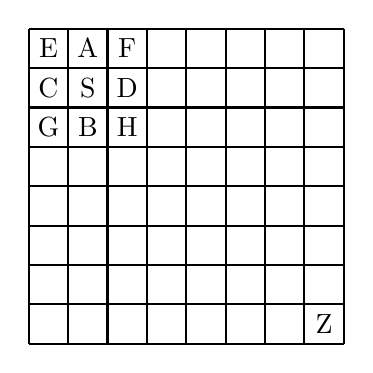
\begin{tikzpicture}
	\draw[step=0.5 cm,black,thick,] (-2,-2) grid (2,2);
	\node at (-1.25,+1.25) {S};
	\node at (-1.25,+1.75) {A};
	\node at (-1.25,+0.75) {B};
	\node at (-1.75,+1.25) {C};
	\node at (-0.75,+1.25) {D};
	\node at (-1.75,+1.75) {E};
	\node at (-0.75,+1.75) {F};
	\node at (-1.75,+0.75) {G};
	\node at (-0.75,+0.75) {H};
	\node at (+1.75,-1.75) {Z};
	\end{tikzpicture}

\end{center}

\hangindent=0.5cm
\parindent=0.5cm
As you can see from the calculations above if the agent moves in the southeast direction then the manhattan distance is greater than the sum of the step cost and estimated cost of traveling to the target cell from the new cell. This means that if the agent is allowed to move in all 8 directions, (north, south, west, east, northeast, souteast, northwest, and southwest), then the triangle inequality defined above does not hold true for every action and that the heuristic value is overestimated. However, as seen in the calculations above if you were to restrict the movement so that the agent can only move in either north, south, west, or east direction then the triangle inequality does hold true for the each of those actions and the heurstic values would not be overestimated. Therefore, the manhattan distance is only consistent when the agent only moves in the four compass directions. Furthermore, the same argument holds true for all applications of the manhattan distances. That is because if an agent were to move in diagonal directions, then the heuristic value of that cell will always be an overestimate. 

\noindent
\textbf{\textit{Prove that adaptive A* leaves initially consistent h-values consistent even if action costs can increase.}}

\hangindent=0.5cm
Let $h(s)$ represent the manhattan distance and $h_{new}(s)$ represent the updated heuristic value calculated by $g(s_{goal}) - g(s)$. In order for an h value to be consistent it has to satisfy the following condition: 
\[\forall (n,a,n'): h(s \leq c(s,a,s') + h(s')$$
In the problem above, we proved that the manhattan distances are consistent. For this problem assuming that the agent only moves in the 4 compass directions, we will prove that the updated heuristic value is also consistent.
\[h_{new}(s) \leq c(s,a,s') + h_{new}(s')$$
\[g(s_{goal}) - g(s) \leq c(s,a,s') + g(s_{goal}) - g(s')$$
\[- g(s) \leq c(s,a,s') - g(s')$$
\[g(s) \geq g(s') - c(s,a,s') $$
After substituting $g(s_{goal}) - g(s)$ for $h_{new}(s)$ and simplifying the inequality, we end up with the following inequality: $g(s) \geq g(s') - c(s,a,s')$. Conceptually this means that as you get closer to the goal state your heuristic value decreases because you are closer to the goal state. Even mathematically the above inequality holds true because $g(s')$ will always be less than $g(s)$. Thus, $h_{new}(s)$ is consistent.  Furthermore, since $h_{new}(s)$ is consistent, even if the action cost increases it will remain consistent. This can easily be shown using the following inequality derived above: $g(s) \geq g(s') - c(s,a,s')$. In this inequality if the action cost were to increase, the right side of the inequality would further decrease. Since $g(s)$ was already greater than $g(s') - c(s,a,s')$, even if the right side of the equation decreases $g(s)$ will still be greater than $g(s') - c(s,a,s')$. As a result $h_{new}(s)$ will always be less than $c(s,a,s') + h_{new}(s')$ because in this case the right side would increase. Thus, even if the action cost increases $h_{new}(s)$ will always be consistent. 

\noindent

\pagebreak
\section*{Part 5: Heuristics in the Adaptive A*}
\textbf{\textit{Implement and compare Repeated Forward A* and Adaptive A* with respect to their runtime. Explain your observations in detail, that is, explain what you observed and give a reason for the observation}}


\begin{center}
\includegraphics{Part5}
\end{center}

Comparing the runtimes of Repeated Forward A* and Adaptive A*, we see that Adapted A* has the fastest runtime on average. Adaptive A* uses A* to repeatedly find shortest path from the current start to the goal. This algorithm updates the h-values of the states to make this larger and make the A* searches more focused. The amount of cell expansion is smaller than Repeated Forward A*. Considering both algorithms breaking ties at higher g-values, they are implemented based on the number of expanded nodes and their runtime.

\pagebreak
\section*{Part 6: Memory Issues}
\textbf{\textit{Suggest Additional ways to reduce the memory consumption of your implementations further}}
\\
\hangindent=0.5cm
In our implementation we stored the g scores and h scores, both of which used around 4 bytes per node. We also stored the x and the y values corresponding to the grid (about 2 bytes each), a node pointer refering to the parent (about 4 bytes), f scores (about 4 bytes), pointers for the final path(about 4 bytes), and a boolean value for the visited cells (about 1 byte) .In total for each node we stored about 25 bytes of data. For the entire implementation, which has 10,201 nodes there was about 255,025 bytes of data stored. As stated in the assignment sheet we can reduce our memory in our implementation by using only 2 bits/cell for pointers. Another way that we can further reduce the memory consumption is to not store f-values for all the cells and calculate them as we go. We can also store g values as we go so that it only stores the g values of the visited cells instead of storing it for all of the cells.  

\noindent
\textbf{\textit{Calculate the amount of memory that they need to operate on gridworlds of size 1001 $\times$ 1001 and the largest gridworld that they can operate on within a memory limit of 4 MBytes.}}

\hangindent=0.5cm
\begin{center}
1 node $\rightarrow $25 bytes of memory \\
1001 x 1001 grid $\rightarrow$ 1,002,001 cells \\
25 bytes/cell $\times$ 1,002,001 cells = 25,050,025 bytes = 25 Megabytes \\
For a grid the size of 1001 x 1001, they would need about 25 Megabytes of memory.
\end{center}

\begin{center}
4 Megabytes = 4,000,000 bytes\\
4,000,000 bytes/25 bytes/cell = 160,000 cells\\
$\sqrt[2]{160,000} = 400$\\
The largest gridworld that they can operate on within a memory limit of 4 MBytes is a 400 x 400 grid.  
\end{center}

\end{document}   